مقالاتی که در فصل‌های قبل‌تر معرفی شد بیشتر در سطح دسته\LTRfootnote{bag} عمل می‌کنند. بدین معنی که در هنگام آموزش
برای آن که نویز حاصل از برچسب‌زنی با روش نظارت از راه دور را کم کنند، تمامی جملاتی را که برچسب رابطه یکسان دارند
و همچنین شامل دو موجودیت مد نظر هستند به صورت یکجا برای استخراج ویژگی‌ها استفاده می‌کنند.

مقالاتی که بر طبق روش بالا عمل می‌کنند از روش‌های مختلفی ارزیابی می‌شوند. برای ارزیابی این روش‌ها از روشی موسوم به نام
«بسط»\LTRfootnote{hold out} استفاده می‌شود. در این روش نیمی از نمونه جملات متناظر
هر رابطه را به عنوان داده آموزشی و نیم دیگر را به عنوان داده آزمون در نظر می‌گیرند. از معیار‌های مختلفی نظیر
منحنی دقت-بازیابی\LTRfootnote{precision-recall curve}، سطح زیر نمودار\LTRfootnote{area under the curve}
و روشی به نام \lr{P@N} ،برای بررسی عملکرد مدل روی داده‌های آزمون استفاده می‌کنند. علاوه بر این معیار‌ها
گاهی عامل انسانی نیز برای ارزیابی عملکرد مدل استفاده می‌شود.

در مقالاتی که بر اساس تک جمله کار می‌کنند یعنی هم در مرحله آموزش و هم در مرحله آزمون از تک جمله
بهره می‌گیرند از معیار‌هایی نظیر دقت\LTRfootnote{Precision}، بازیابی\LTRfootnote{Recall}
و \lr{F1} برای ارزیابی کار خود استفاده می‌کنند.

در ادامه نتایج مقالات را بر طبق معیار‌های معرفی شده ارائه کرده و مقایسه می‌کنیم.
در این جا برای سادگی، مدل‌های ارائه شده را با نام مخفف انگلیسی آن‌ها اسم می‌بریم.
در ادامه اسم مخفف هر یک از مقالات معرفی می‌شود.

\begin{itemize}
    \item \lr{EA-GPCNN}: شبکه عصبی پیچشی تکه‌ای با تاکید بر موجودیت‌ها
    \item \lr{PCNN-PATT+SBA}: شبکه عصبی پیچشی تکه‌ای با توجه مکانی و توجه به دسته‌های مشابه
    \item \lr{PLSTM-CNN}: شبکه عصبی پیچشی کوتاه‌مدت بلند تکه‌ای
    \item \lr{BERT-PCNN}: شبکه عصبی پیچشی تکه‌ای بر پایه مدل برت\LTRfootnote{BERT}
\end{itemize}

سه مقاله اول در هنگام آموزش بر اساس ویژگی‌هایی که از دسته استخراج کرده‌اند آموزش می‌بینند
در حالی که روش آخر یعنی همواره \lr{BERT-PCNN} در سطح جمله عمل می‌کند. بنابراین سه روش اول را به صورت جدای
از روش آخر بررسی خواهیم کرد.

نمودار دقت-بازیابی برای سه روش \lr{EA-GPCNN}، \lr{PCNN-PATT+SBA} و \lr{PLSTM-CNN} در شکل \ref{recall_precision}
مشاهده می‌شود. همان‌طور که مشاهده می‌شود متاسفانه هیچ یک از مقالات نتیجه خود را با نتیجه مقاله دیگر مقایسه نکرده است،
بنابراین این روش‌ها را صرفا می‌توان از روی شکل ارائه شده با هم مقایسه کرد. بر اساس شکل‌ها عملکرد روش \lr{EA-GPCNN}
از دو روش دیگر بهتر است چرا که بر طبق نمودار به ازای مقادیر یکسان بازیابی نتایج بهتری برای دقت ارائه کرده است.

\begin{figure}[h]
    \begin{subfigure}{0.3\linewidth}
        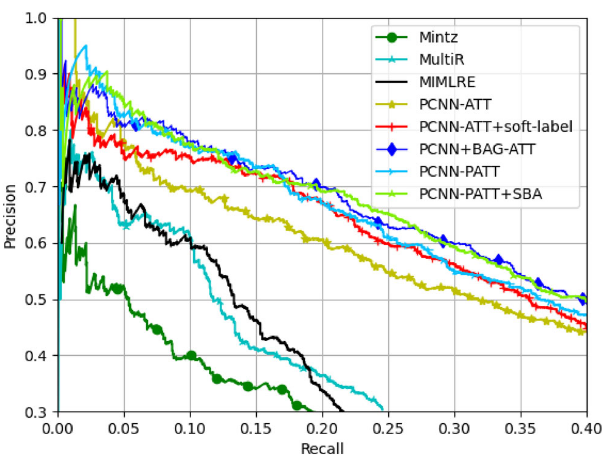
\includegraphics[width=\linewidth]{images/pos_attension/performance.png}
        \caption{عملکرد مدل \lr{PCNN-PATT+SBA}}
    \end{subfigure}
    \begin{subfigure}{0.3\linewidth}
        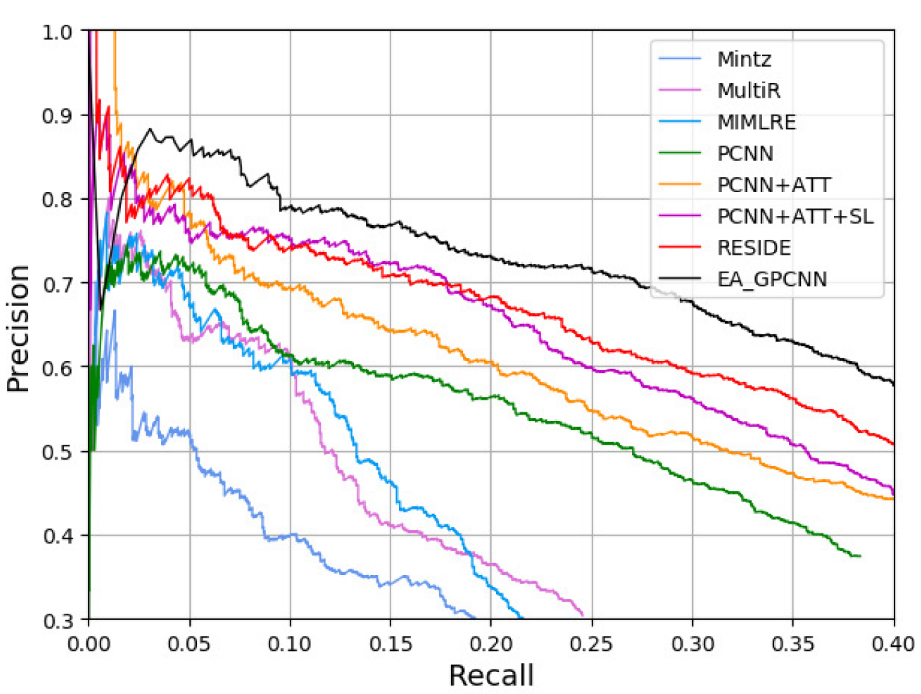
\includegraphics[width=\linewidth]{images/gated/performance.png}
        \caption{عملکرد مدل \lr{EA-GPCNN}}
    \end{subfigure}
    \begin{subfigure}{0.3\linewidth}
        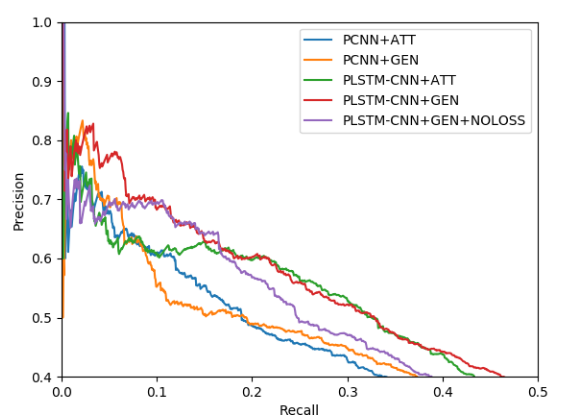
\includegraphics[width=\linewidth]{images/shared/nyt_dataset.png}
        \caption{عملکرد مدل \lr{PLSTM-CNN}}
    \end{subfigure}
    \caption{بررسی عملکرد سه روش \lr{EA-GPCNN}، \lr{PCNN-PATT+SBA} و \lr{PLSTM-CNN} در مجموعه داده نیویورک تایمز}
    \label{recall_precision}
\end{figure}

روش دیگری که این سه مدل را می‌توان بررسی کرد روشی به نام \lr{P@N} است. در این روش دقت عملکرد مدل به ازای
$N$ نمونه آزمون بررسی می‌شود نتایج این بررسی در جدول \ref{pn} مشاهده می‌شود. همان‌طور که مشاهده می‌شود در این معیار
ارزیابی نیز روش \lr{EA-GPCNN} برتر از دو روش دیگر عمل کرده است.

\begin{latin}
\begin{table}[h]
    \centering
    \caption{\rl{بررسی عملکرد سه روش \lr{EA-GPCNN}، \lr{PCNN-PATT+SBA} و \lr{PLSTM-CNN} در مجموعه داده نیویورک تایمز بر معیار \lr{P@N}}}
    \label{pn}
    \begin{tabular}{c|c|c|c|c}
        P@N & 100 & 200 & 300 & mean \\
        \hline
        EA-GCPNN & 91 & 87.5 & 82.0 & 86.8 \\
        PLSTM-CNN & 76.3 & 65.6 & 60.2 & 67.4 \\
        PCNN-PATT+SBA & 86 & 81 & 76.7 & 81.2
    \end{tabular}
\end{table}
\end{latin}

بر طبق معیار‌های ارزیابی بالا بهترین روش \lr{EA-GCPNN} است. این روش بازنمایی هر کلمه را بر اساس فاصله آن از موجودیت
وزن‌دهی می‌کند. در مقام بعدی روش \lr{PCNN-PATT+SBA} است که از مکانیزم توجه استفاده کرده و
دسته‌های با ویژگی‌های مشابه را در هم ادغام می‌کرد. در نهایت روش \lr{PLSTM-CNN} است که از شبکه عصبی \lr{LSTM}
برای بهبود کدگذاری ارائه شده توسط \lr{PCNN} بهره می‌برد. این نتایج نشان از اهمیت دخیل کردن بازنمایی موجودیت در
بازنمایی سایر کلمات دارد چرا که روش‌هایی که به این بخش بیشتر اهمیت داده‌اند نتایج بهتری گرفته‌اند.

تا به این جا نتایج عملکرد سه مدل \lr{EA-GPCNN}، \lr{PCNN-PATT+SBA} و \lr{PLSTM-CNN} را با هم مقایسه کردیم.
در ادامه می‌خواهیم نتایج عملکرد مدل \lr{BERT-PCNN} که رویکرد متفاوتی نسبت به روش‌های نامبرده دارد را
بررسی می‌کنیم.

ارزیابی روش \lr{BERT-PCNN} بر روی مجموعه داده‌های \lr{SemEval-2010} و \lr{SemEval-2018} انجام شده است.
این مدل می‌تواند روی مجموعه داده \lr{SemEval-2010} به نتیجه $89.95$ درصد روی معیار \lr{F1} برسد. عملکرد مدل روی مجموعه داده
\lr{SemEval-2018} از این هم بهتر بوده و توانسته به نتیجه $99.52$ روی معیار \lr{F1} برسد.
به نظر می‌رسد که نتیجه بهتر روی مجموعه داده \lr{SemEval 2018} به خاطر خود مجموعه داده باشد چرا که در
مقاله توضیحی در بابت اختلاف نتایج داده نشده است.